%\documentclass{beamer}
%\usetheme{Ilmenau}

\documentclass[a4,portraitt]{slides}
\usepackage{biggy,graphics,times,epsfig}

\usepackage{hyperref}

%\documentclass[biggy]{slides}

%\documentstyle[graphics,biggy,times,epsfig]{slides}
%\documentstyle[12pt,a4wide,times]{article}


%\setlength{\parindent}{0in}
%\setlength\textheight{\textheight \times 0.5}

\title{Chapter One}

\begin{document}

\begin{center}
{\Large
Programming in C
}

Dr. Neill Campbell

Room 3.14 MVB

Neill.Campbell@bristol.ac.uk\\[1em]
{\small
\verb^http://www.cs.bris.ac.uk/^
}
\end{center}

\section*{About the Course}

{\footnotesize
The course notes were originally based on:\\
{\it
C By Dissection (3rd edition)\\
Al Kelley and Ira Pohl\\
}
because I liked arrays being taught later.
}

\newpage
\subsection*{Resources}
\begin{itemize}
\item Free : \url{https://en.wikibooks.org/wiki/C_Programming}
\item A list of more : \url{https://www.linuxlinks.com/excellent-free-books-learn-c/}
\item Whatever you use, make sure it's {\bf ANSI C} that's being taught, not something else e.g. C11 or C++.
\end{itemize}

\newpage
\subsection*{K\&R}
If you fall in love with C and  know you're going to use it for the rest of your life, the reference `bible' is K\&R 2nd edition.
It's not a textbook for those new to programming, though.
\begin{figure}[h]
\centerline{
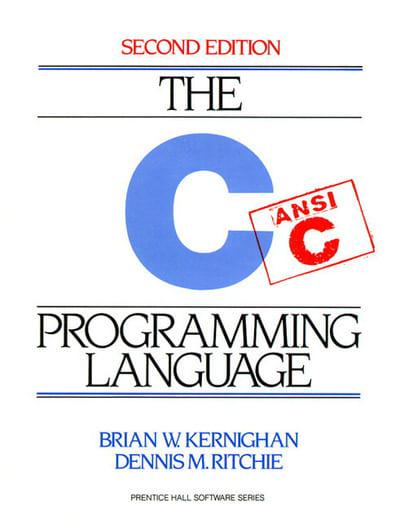
\includegraphics[scale=0.65]{../Figs/9780131103627.jpg}
}
\end{figure}

\newpage
\subsection*{Computer Science Ethos}
\begin{itemize}
\item Talk to your friends, ask for help, work together.
\item Never pass off another persons work as your own.
\item Do not pass work to others - either on paper or
electronically.
\item If someone takes your code and submits it, we need to investigate where it originated.
\item Be careful of placing your code on publicly accessible sites e.g. github.
\end{itemize}

\newpage
\subsection*{History of C}
{\samepage
\begin{center}
\begin{figure}[h]
\centerline{
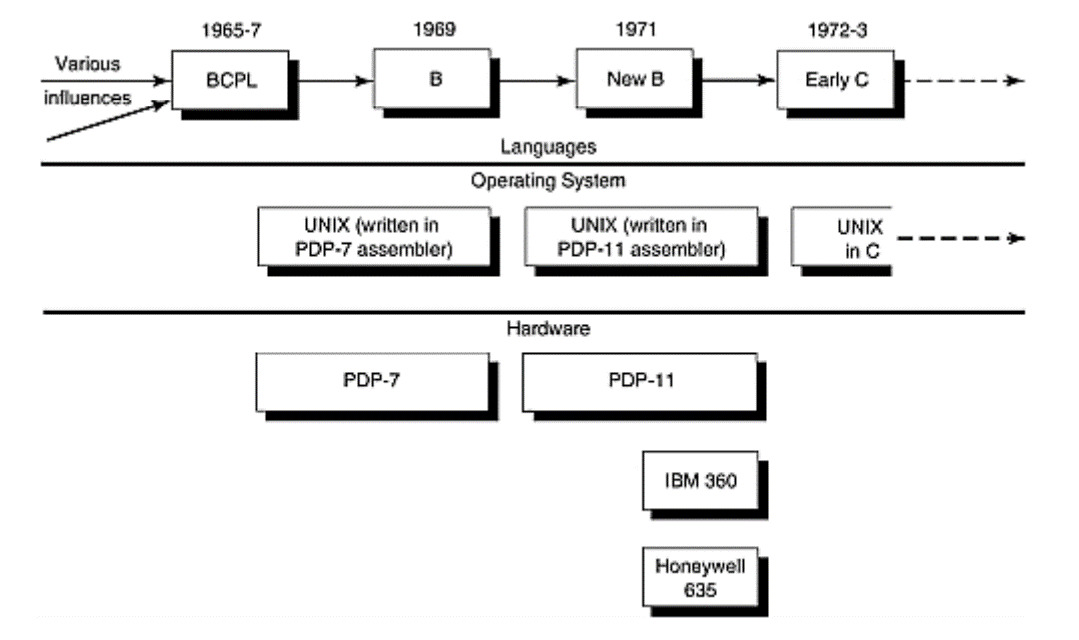
\includegraphics[scale=0.5]{../Figs/evolvec.jpg}
}
\end{figure}
\end{center}
{\small
From {\it Deep C Secrets} by Peter Van Der Linden
}}

\newpage
\subsection*{History of C}
\begin{itemize}
\item BCPL - Martin Richards
\item B - Ken Thomson 1970
\item Both of above are {\em typeless}.
\item C - Dennis Ritchie 1972 designed for\\(\& implemented on) a UNIX system.
\item K\&R C (Kernighan and Ritchie) 1978
\item ANSI C (COMSM1201)
\item C++ - Object Oriented Programming (OOP)
\item Java (Subset of C++, WWW enabled).
\end{itemize}

\subsection*{Why C ?}
\begin{itemize}
\item Low-level (c.f. Java)
\item Doesn't hide nitty-gritty
\item Fast ?
\item Wide acceptability
\item Large parts common to Java
\end{itemize}
\newpage

\newpage
\subsection*{Programming and Software Engineering}
\begin{itemize}
\item Was traditionally Lectured 2(or 3) hours a week for weeks 1-12 
\item With COVID-19 I'll post the equivalent online, broken
into manageable chunks
\item Programming (C), data structures, algorithms - searching, sorting, string processing, trees etc.
\end{itemize}

\newpage
\subsection*{Assessment}
\begin{itemize}
\item Weekly (unmarked) exercises that, if completed, should ensure you are able to pass the unit.
\item Approximately three/four assignments and one lab test.
\item One major project due in early TB2 (35\%).
\item Hard to gauge timings, so don't make any plans in advance -
I'll change it if we're going too fast.
\end{itemize}

\newpage
{\samepage
\subsection*{Help with Computers}
\begin{itemize}
\item Any problems with the computers e.g. installing the correct S/W, accessing lab machines: \url{http://www.bris.ac.uk/it-services/}.
\item They are also the people to see about passwords etc.
\item This page also links to the rather useful Laptop \& Mobile Clinic.
\end{itemize}
}

\newpage
{\samepage
\subsection*{Help with the Unit}
\begin{itemize}
\item Further information is available via the Blackboard site.
\item Help will mainly be via myself giving `live' Q\&A session, the associated MS Teams group and the corresponding Forum.
\item You will often work in a peer group (approx $15$ people).
\item There will be a group of Teaching Assistants to help each of these groups.
\item TAs are not allowed to write pieces of code for you,
nor undertake detailed bug-fixing of your program.
\end{itemize}
}

\newpage
\section*{A First Program}

\begin{verbatim}
/* The traditional first program
   in honour of Dennis Ritchie
   who invented C at Bell Labs
   in 1972 */

#include <stdio.h>

int main(void)
{
   printf("Hello, world!\n");
   return 0;
}
\end{verbatim}

\newpage
\section*{Dissecting the 1st Program (1)}

\begin{itemize}
\item Comments are bracketed by the {\bf /*} and {\bf */} pair.
\item
\begin{verbatim}
#include <stdio.h>
\end{verbatim}
Lines that begin with a {\bf \#}
are called preprocessing directives.
\item \begin{verbatim}
int main(void)
\end{verbatim}
Every program has a function called \begin{verbatim}
main()
\end{verbatim}

\item Statements are grouped using braces,
\begin{verbatim}
{ ... }
\end{verbatim}
\end{itemize}

\section*{Dissecting the 1st Program (2)}

\begin{itemize}
\item \verb+printf()+ One of the pre-defined library functions being called (invoked) using a single argument the string:
\begin{verbatim}
"Hello, world!\n"
\end{verbatim}
\item The \verb+\n+ means print the single character {\it newline}.
\item Notice all declarations and statements are terminated with a
semi-colon.
\item \verb+return(0)+
Instruct the Operating System that the function
\verb+main()+ has completed successfully.
\end{itemize}

\newpage
\newpage
\section*{The Second Program}

\begin{verbatim}
#include <stdio.h>

int main(void)
{
   int   inches, feet, fathoms;

   fathoms = 7;
   feet = 6 * fathoms;
   inches = 12 * feet;

   printf("Wreck of the Hesperus:\n");
   printf("Its depth at sea in");
   printf(" different units:\n");
   printf("   %d fathoms\n", fathoms);
   printf("   %d feet\n", feet);
   printf("   %d inches\n", inches);
   return 0;
}
\end{verbatim}

\section*{Dissecting the 2nd Program}

\begin{itemize}
\item \verb+#include <stdio.h>+ Always required when using I/O.
\item \verb+int inches, feet, fathoms;+ {\it Declaration}
\item \verb+fathoms = 7;+ {\it  Assignment }
\item \verb+printf()+has 2 Arguments.
The {\it control string}
contains a \verb+%d+ to indicate an integer is to be\\ printed.
\end{itemize}

\begin{verbatim}
preprocessing directives

int main(void)
{
   declarations

   statements
}
\end{verbatim}
\newpage
\section*{ Arithmetic Operators }

\begin{itemize}
\item \verb^+ , - , / , *, %^
\item Addition, Subtraction, Division, Multiplication,\\ Modulus.
\item Integer arithmetic discards remainer i.e.\\
\verb+1/2+ is 0 , \verb+7/2+ is 3.
\item Modulus (Remainder) Arithmetic.\\
\verb+7%4+ is 3, \verb+12%6+ is 0.

\item
Only available for integer arithmetic.
\end{itemize}

\newpage
\section*{ The Character Type }

\begin{itemize}
\item The  keyword \verb+char+ stands for character.

\item Used with single quotes i.e.
\verb^'A'^,
\verb^'+'^.

\end{itemize}

\begin{verbatim}
#include <stdio.h>

int main(void)
{
   char   c;

   c = 'A';
   printf("%c\n", c);
   return 0;
}
\end{verbatim}

\begin{itemize}
\item The letter A is printed.
\item Note the \verb+%c+ conversion format.
\end{itemize}

\newpage
\section*{ Floating Types }


\begin{itemize}
\item In ANSI C there are three floating types:
    \begin{enumerate}
        \item \verb+float+
        \item \verb+double+
        \item \verb+long double+
    \end{enumerate}
\item The {\it Working Type} is doubles.
\end{itemize}

\begin{small}
\begin{verbatim}
#include <stdio.h>

int main(void)
{
   float   x, y;

   x = 1.0;
   y = 2.0;
   printf("Sum of x & y is %f.\n", x + y);
   return 0;
}
\end{verbatim}
\end{small}

\section*{The Preprocessor}

\begin{itemize}
\item A \verb+#+ in the first column signifies
a preprocessor statement.

\item \verb+#include <file.h>+
Exchange this line for
the entire contents of \verb+file.h+,
which is to be found in a standard place.

\item \verb+#define ROUGH_PI (22.0/7.0)+
\\  Replace all occurrences of \verb+ROUGH_PI+
with\\ \verb+ (22.0/7.0)+.

\item
Include files generally contain other \verb+#define+'s
and \verb+#include+'s.

\end{itemize}

\newpage
\section*{Using printf()}

\begin{itemize}
\item \verb+printf( fmt-str, arg1, arg2, ...);+

\end{itemize}

\begin{center}
\begin{tabular}{|c|l|} \hline
\verb+%c+   & Characters \\ \hline
 \verb+%d+  & Integers \\ \hline
 \verb+%e+  & Floats/Doubles (Engineering Notation) \\ \hline
 \verb+%f+  & Floats/Doubles \\ \hline
 \verb+%s+  & Strings \\ \hline
\end{tabular}
\end{center}

\begin{itemize}
\item Fixed-width fields: \verb+printf("F:%7f\n", f);+ \\
\verb+F: 3.0001+

\item Fixed Precision: \verb+printf("F:%.2f\n", f);+\\
\verb+F:3.00+
\end{itemize}

\newpage
\section*{Using scanf()}

\begin{itemize}
\item Similar to \verb+printf()+ but deals with
{\it input} rather than {\it output}.

\item \verb+scanf(fmt-str, &arg1, &arg2, ...);+

\item Note that the {\it address} of the argument is required.

\end{itemize}

\begin{center}
\begin{tabular}{|c|l|} \hline
\verb+%c+   & Characters \\ \hline
\verb+%d+   & Integers \\ \hline
\verb+%f+   & Floats \\ \hline
\verb+%lf+  & Doubles \\ \hline
\verb+%s+   & Strings \\ \hline
\end{tabular}
\end{center}

\begin{itemize}
\item Note doubles handled differently than floats.

\end{itemize}

\newpage
\section*{ The {\tt while} Loop }

\begin{small}
{\bf
\begin{verbatim}
while (test is true) {
    statement 1;
        ...
    statement n;
}
\end{verbatim}
}

\begin{verbatim}
/* Sums are computed. */
#include <stdio.h>

int main(void)
{
   int     cnt = 0;
   float   sum = 0.0, x;

   printf("Input some numbers:  ");
   while (scanf("%f", &x) == 1) {
      cnt = cnt + 1;
      sum = sum + x;
   }
   printf("\n%s%5d\n%s%12f\n\n",
      "Count:", cnt,
      "  Sum:", sum);
   return 0;
}
\end{verbatim}
\end{small}

\newpage
\section*{Common Mistakes}

\subsubsection*{Missing "}
\begin{verbatim}
printf("%c\n, ch);
\end{verbatim}

\subsubsection*{Missing ;}
\begin{verbatim}
a = a + 1
\end{verbatim}

\subsubsection*{Missing Address in {\tt scanf()}}
\begin{verbatim}
scanf("%d", a);
\end{verbatim}

\newpage
\begin{center}
{\Large Chapter Two \\ Operators}
\end{center}

\section*{Grammar}


\begin{itemize}
\item  C has a grammar/syntax like every other language.
\item  It has {\it Keywords}, {\it Identifiers}, {\it Constants}, {\it String Constants}, {\it Operators} and {\it Punctuators}.
\item
Valid Identifiers :\\
\verb^k^,
\verb^_id^,
\verb^iamanidentifier2^,
\verb^so_am_i^.
\item  {\bf Invalid} Identifiers :\\
\verb^not#me^,
\verb^101_south^,
\verb^-plus^.
\item  Constants :\\
\verb^17^ (decimal),
\verb^017^ (octal),
\verb^0x17^ (hexadecimal).
\item  String Constant enclosed in double-quotes:\\
\verb^"I am a string"^
\end{itemize}

\section*{Operators}

\begin{itemize}
\item All operators have rules of both {\it precedence}
and {\it associativity}.
\item  \verb^1 + 2 * 3^ is the same as
\verb^1 + (2 * 3)^ because \verb^*^ has
a higher precedence than \verb^+^.
\item  The associativity of \verb^+^ is left-to-right, thus\\
\verb^1 + 2 + 3^ is equivalent to
\verb^(1 + 2) + 3^.
\item  Increment and decrement operators:\\
\verb^i++;^ is equivalent to \verb^i = i + 1;^
\item  May also be prefixed \verb^--i;^
\end{itemize}
\begin{verbatim}
int a, b, c = 0;
a = ++c;
b = c++;
printf("%d %d %d\n", a, b, ++c);
\end{verbatim}

\section*{Assignment}

\begin{itemize}
\item  The \verb^=^ operator has a low precedence
and a right-to-left associativity.
\item  \verb^a = b = c = 0; ^ is valid and equivalent to:\\
\verb^a = (b = (c = 0));^
\item  \verb^i = i + 3;^ is the same as \verb^i += 3;^
\item  Many other operators are possible e.g.\\\\ \verb^-=, *=, /=^.
\end{itemize}

\newpage
\section*{The Power of 2 Program}



\begin{verbatim}
/* Some powers of 2 are printed. */

#include <stdio.h>

int main(void)
{
   int   i = 0, power = 1;

   while (++i <= 10)
      printf("%5d", power *= 2);
   printf("\n");
   return 0;
}
\end{verbatim}

The output is:

{\tiny
\begin{verbatim}
    2    4    8   16   32   64  128  256  512 1024
\end{verbatim}
}

\newpage
\section*{Random Numbers}

\begin{verbatim}
#include <stdio.h>
#include <stdlib.h>

int main(void)
{
   int   i, n;

   printf("\n%s\n%s",
    "Randomly distributed integers"
    "are printed." ,
    "How many do you want to see?  ");
   scanf("%d", &n);
   for (i = 0; i < n; ++i) {
      if (i % 4 == 0)
         printf("\n");
      printf("%12d", rand());
   }
   printf("\n");
   return 0;
}
\end{verbatim}

\section*{The Standard Library}


The output is:

{\tiny
\begin{verbatim}
Some randomly distributed integers will be printed.
How many do you want to see?  11

    16838     5758    10113    17515    31051     5627
    23010     7419    16212     4086     2749
\end{verbatim}
}

\begin{itemize}
\item Definitions required for the proper use of
many functions such as\\ \verb^rand()^
are found in \verb^stdlib.h^.
\item  Do not mistake these header files for the libraries
themselves !
\end{itemize}

\newpage
\begin{center}
{\Large Chapter Three \\ Flow Control}
\end{center}

\section*{Relations}

\begin{center}
\begin{tabular}{|l|l|} \hline
\verb^<^    & less than             \\ \hline
\verb^>^    & greater than          \\ \hline
\verb^<=^   & less than or equal to     \\ \hline
\verb^>=^   & greater than or equal to  \\ \hline
\verb^==^   & {\bf equal to}        \\ \hline
\verb^!=^   & not equal to          \\ \hline
\verb^!^    & not               \\ \hline
\verb^&&^   & logical and           \\ \hline
\verb^||^   & logical or            \\ \hline
\end{tabular}
\end{center}

\newpage
\section*{True and False}

\begin{itemize}
\item Any relation is either {\it true} or {\it false}.
\item Any non-zero value is {\it true}.
\item \verb^(a < b)^ returns the value {\it 0} or {\it 1}.
\item \verb^(i == 5)^ is a {\bf test} not an {\bf assignment}.
\item \verb^(!a)^ is either {\it true (1)} or {\it false (0)}.
\item \verb^(a && b)^ is {\it true} if both \verb^a^ and \verb^b^ are {\it true}.
\end{itemize}

\newpage
\section*{Short-Circuit Evaluation}

\begin{verbatim}
if(x >= 0.0 && sqrt(x) < 10.0){

..... /* Do Something */

}
\end{verbatim}

The \verb^sqrt()^ statement is never reached if the first test is {\it false},
since in a logical AND, once any expression is {\it false} the whole must
be {\it false}.


\newpage
\section*{The {\tt if()} Statement}

\begin{verbatim}
if (expr)
   statement
\end{verbatim}

If more than one statement is required:

\begin{verbatim}
if (expr) {
   statement-1
       .
       .
       .
   statement-n
}
\end{verbatim}

\newpage
Adding an \verb^else^ statement:

\begin{verbatim}
if (expr) {
   statement-1
       .
       .
       .
   statement-n
}
else{
   statement-a
       .
       .
       .
   statement-e
}
\end{verbatim}

\newpage
A practical example:

\begin{verbatim}
#include <stdio.h>

int main(void)
{
   int   x, y, z, min;

   printf("Input three integers:  ");
   scanf("%d%d%d", &x, &y, &z);
   if (x < y)
      min = x;
   else
      min = y;
   if (z < min)
      min = z;
   printf("The minimum value is " \
          "%d\n", min);
   return 0;
}
\end{verbatim}

\section*{The {\tt while()} Statement}

\begin{verbatim}
while(expr)
   statement
\end{verbatim}

This, as with the \verb^for^ loop, may execute compound statements:

\begin{verbatim}
while(expr){
   statement-1
       .
       .
       .
   statement-n
}
\end{verbatim}

\section*{The {\tt for()} Loop}

This is one of the more complex and heavily used means
for controlling execution flow.

\begin{verbatim}
for( init ; test; loop){
   statement-1
       .
       .
       .
   statement-n
}
\end{verbatim}

\newpage
and may be thought of as:
\begin{verbatim}
init;
while(test){
   statement-1
       .
       .
       .
   statement-n
   loop;
}
\end{verbatim}

In the \verb^for()^ loop, note:
\begin{itemize}
\item Semi-colons separate the three parts.
\item Any (or all) of the three parts could be empty.
\item If the test part is empty, it evaluates to {\it true}.\\
\verb^for(;;){ a+=1; }^  is an infinite loop.
\end{itemize}

\newpage
{\samepage
\begin{verbatim}
/* Find triples of integers that
   add up to N.                  */

#include <stdio.h>

#define   N   7

int main(void)
{
   int   cnt = 0, i, j, k;

   for (i = 0; i <= N; i++)
      for (j = 0; j <= N; j++)
       for (k = 0; k <= N; k++)
          if (i + j + k == N) {
             ++cnt;
             printf("%3d%3d%3d\n",
                    i, j, k);
          }
   printf("\nCount: %d\n", cnt);
   return 0;
}
\end{verbatim}
}
\newpage
The result is:

{\tiny
\begin{verbatim}
  0  0  7
  0  1  6
  0  2  5
  0  3  4
  0  4  3
  0  5  2
  0  6  1
  0  7  0
  1  0  6
  1  1  5
  1  2  4
  1  3  3
  1  4  2
  1  5  1
  1  6  0
  2  0  5
  2  1  4
  2  2  3
  2  3  2
  2  4  1
  2  5  0
  3  0  4
  3  1  3
  3  2  2
  3  3  1
  3  4  0
  4  0  3
  4  1  2
  4  2  1
  4  3  0
  5  0  2
  5  1  1
  5  2  0
  6  0  1
  6  1  0
  7  0  0
\end{verbatim}
}

\section*{The Comma Operator}

This has the lowest predence of all the operators in C
and associates left to right.

\begin{verbatim}
a = 0 , b = 1;
\end{verbatim}

Hence, the \verb^for^ loop may become quite complex :

\begin{verbatim}
for(sum = 0 , i = 1; i <= n; ++i)
   sum += i;
\end{verbatim}

An equivalent, but more difficult to read expression :

{\small
\begin{verbatim}
for(sum = 0 , i = 1; i <= n; ++i, sum += i);
\end{verbatim}
}

\begin{itemize}
\item Notice the loop has an empty body, hence the semicolon.
\end{itemize}

\newpage
\section*{The {\tt do-while()} Statement}

\begin{verbatim}
do {
   statement-1
       .
       .
       .
   statement-n
} while ( test );
\end{verbatim}

Unlike the \verb^while()^ loop, the \verb^do-while()^ will always
be executed at least once.

\newpage
\section*{The {\tt switch()} Statement}

\begin{verbatim}
switch (val) {
   case 1 :
      a++;
      break;
   case 2 :
   case 3 :
      b++;
      break;
   default :
      c++;
}
\end{verbatim}

\begin{itemize}
\item The \verb^val^ must be an integer.
\item The \verb^break^ statement causes execution to jump out
of the loop. No \verb^break^ statement causes execution to
`fall through' to the next line.
\item The \verb^default^ label is a catch-all.
\end{itemize}

\newpage
\section*{The Conditional Operator}

\begin{verbatim}
expr1 ? expr2 : expr3
\end{verbatim}

If \verb^expr1^ is {\it true} then \verb^expr2^ is executed, else
\verb^expr3^ is evaluated, i.e.:

\verb^x = ((y < z) ? y : z);^

\newpage
\begin{center}
{\Large Chapter Four \\ Functions}
\end{center}

\begin{verbatim}
#include <stdio.h>

int   min(int a, int b);

int main(void)
{
   int   j, k, m;

   printf("Input two integers:  ");
   scanf("%d%d", &j, &k);
   m = min(j, k);
   printf("\nOf the two values " \
          " %d and %d, " \
          "the minimum is %d.\n\n",
          j, k, m);
   return 0;
}
\end{verbatim}

\newpage

\begin{verbatim}
int min(int a, int b)
{
   if (a < b)
      return a;
   else
      return b;
}
\end{verbatim}

\begin{itemize}
\item Execution begins, as normal, in the \verb^main()^ function.
\item The function {\it prototype is shown} at the top of the file.
This allows the compiler to check the code more thoroughly.
\item The function \verb^min()^ returns an \verb^int^ and takes
two \verb^int^'s as arguments.
\item The function is defined between two braces.
\item The \verb^return^ statement is used return a value
to the calling statement.
\item A function which has no return value, is declared \verb^void^
and is equivalent to a procedure.
\end{itemize}

\section*{Assert}

The assert macro is defined in the header file\\ \verb^assert.h^.
This is used to ensure the value of an expression is as we
expect it to be.

\newpage
\begin{verbatim}
#include <assert.h>

double f(int a, int b)
{

   double x;

   assert(a > 0);

   /* precondition */
   assert(b >= 7 && b <= 11);

      .
      .
      .

   /* postcondition */
   assert(x >= 1.0);

   return(x);
}
\end{verbatim}

\begin{itemize}
\item If an assertion fails, an error is printed and the
program is aborted.
\item By \verb^#define^'ing \verb^NDEBUG^ all assertions are
ignored, allowing them to be used during development and switched
off later.
\end{itemize}

\newpage
\section*{Program Layout}
{\samepage
It is common for the \verb^main()^ function to come
first in a program :
\begin{verbatim}
#include <stdio.h>
#include <stdlib.h>

list of function prototypes

int main(void)
{
   . . . . .
}

int f1(int a, int b)
{
   . . . . .
}

int f2(int a, int b)
{
   . . . . .
}
\end{verbatim}
}

\newpage
However, it is possible to avoid the need for function prototypes
by defining a function before it is used :

\begin{verbatim}
#include <stdio.h>
#include <stdlib.h>

int f1(int a, int b)
{
   . . . . .
}

int f2(int a, int b)
{
   . . . . .
}

int main(void)
{

   . . . . .

}
\end{verbatim}

\newpage
\section*{Call by Value}

In the following example, a function is passed an integer
using call by value:

\begin{verbatim}
#include <stdio.h>

void fnc1(int a);

int main(void)
{

   int x = 1;

   fnc1(x);
   printf("%d\n", x);

}
\end{verbatim}
\newpage
\begin{verbatim}
void fnc1(int a)
{

   a = a + 1;

}
\end{verbatim}

The function does not change the value of \verb^x^ in\\
\verb^main()^, since \verb^a^ in the function is effectively
only a {\bf copy} of the variable.

\newpage
\section*{Multiply}
Write a simple function \verb^int mul(int a, int b)^ which
multiples two integers together {\b without} the use of the
multiply symbol in C (i.e. the \verb^*^).

Use \verb^assert()^ calls in \verb^main()^ test it thoroughly.

\newpage
\section*{Recursion}

{\samepage
A repeated computation computation is normally
achieved via {\it iteration}, e.g. using \verb^for()^:

\begin{verbatim}
#include <stdio.h>

int fact(int a);

int main(void)
{

   int a, f;

   printf("Input a number :\n");
   scanf("%d", &a);
   f = fact(a);
   printf("%d! is %d\n", a, f);

   return(0);

}
\end{verbatim}
}
\newpage
\begin{verbatim}
int fact(int a)
{

   int i;
   int tot = 1;

   for(i=1; i<=a; i++){
      tot *= i;
   }
   return tot;
}
\end{verbatim}

We could also achieve this via {\it recursion} :

\newpage
{\samepage
\begin{verbatim}
#include <stdio.h>

int fact(int a);

int main(void)
{

   int a, f;

   printf("Input a number :\n");
   scanf("%d", &a);
   f = fact(a);
   printf("%d! is %d\n", a, f);

   return(0);
}

int fact(int a)
{
   if(a > 0)
      return (a*fact(a - 1));
   else
      return 1;

}
\end{verbatim}
}
\newpage
\begin{center}
{\Large Chapter Five \\ Characters}
\end{center}

\section*{Storage of Characters}

\begin{itemize}
\item Characters are stored in the machine as one byte i.e.\ one
of {\bf 256} possible values.
\item These may be thought of a characters, or very small integers.
\item Only a subset of these 256 values are required
for the printable characters, space, newline etc.
\end{itemize}

\newpage
\begin{itemize}
\item Declaration:
\begin{verbatim}
char c;

c = 'A';
\end{verbatim}
or :
\begin{verbatim}
char c1 = 'A', c2 = '*', c3 = ';' ;
\end{verbatim}

The particular integer used to represent a character
is dependent on the encoding used. The most common
of these, used on most UNIX and PC platforms, is ASCII.

\begin{center}
\begin{tabular}{|l|lllll|}\hline
lowercase   & 'a' & 'b' & 'c' & \verb^...^ & 'z' \\
ASCII value & 97  &  98 &  99 & \verb^...^ & 112 \\ \hline
uppercase   & 'A' & 'B' & 'C' & \verb^...^ & 'Z' \\
ASCII value & 65  &  66 &  67 & \verb^...^ &  90 \\ \hline
digit       & '0' & '1' & '2' & \verb^...^ & '9' \\
ASCII value & 48  &  49 &  50 & \verb^...^ &  57 \\ \hline
other       & '\&' & '*' & '+' & \verb^...^ & \\
ASCII value & 38  &  42 &  43 & \verb^...^ & \\ \hline
\end{tabular}
\end{center}

\item When using \verb^printf()^ and \verb^scanf()^ the formats
\verb^%c^ and \verb^%d^ do very different things :
\begin{verbatim}
char c = 'a'
printf("%c\n", c); /* prints : a  */
printf("%d\n", c); /* prints : 97 */
\end{verbatim}

\item Hard-to-print characters have an escape\\ sequence
i.e. to print a newline, the 2 character escape \verb^'\n'^ is used.
\end{itemize}

\newpage
\section*{Using {\tt getchar()} and {\tt putchar()}}

\begin{verbatim}
/* Outputs characters twice */                                                     
#include <stdio.h>

int main(void)
{

   char c;
   while (1) {
      c = getchar();
      putchar(c);
      putchar(c);
   }
   return 0;
}
\end{verbatim}
\newpage

This has the unfortunate problem of never terminating,
a {\tt CTRL-C} would be required.

\begin{verbatim}
#include <stdio.h>

int main(void)
{
   int   c;

   while ((c = getchar()) != EOF) {
      putchar(c);
      putchar(c);
   }
   return 0;
}
\end{verbatim}

The end-of-file constant is defined in {\tt stdio.h}. Although
system dependent, {\tt -1} is often used. On the UNIX system
this is generated when the end of a file being piped is reached,
or when {\tt CTRL-D} is pressed.

\section*{Capitalising}

\begin{verbatim}
/* Outputs characters twice */

#include <stdio.h>

#define CAPS ('A' - 'a')

int main(void)
{
   int   c;

   while ((c = getchar()) != EOF)
      if (c >= 'a' && c <= 'z')
          putchar(c + CAPS);
      else
         putchar(c);
   return 0;
}
\end{verbatim}

\newpage
This is more easily achieved by using some of
the definitions found in {\tt ctype.h}.

\begin{center}
\begin{tabular}{|l|l|} \hline
Macro        & {\tt true} returned if: \\ \hline
isalnum(int c) & Letter or digit \\
isalpha(int c) & Letter \\
iscntrl(int c) & Control character \\
isdigit(int c) & Digit \\
isgraph(int c) & Printable (not space) \\
islower(int c) & Lowercase\\
isprint(int c) & Printable\\
ispunct(int c) & Punctuation\\
isspace(int c) & White Space\\
isupper(int c) & Uppercase\\
isxdigit(int c)& Hexadecimal\\
isascii(int c) & ASCII code \\ \hline
\end{tabular}
\end{center}


Some useful functions are :

\begin{center}
\begin{tabular}{|l|l|} \hline
Function/Macro & Returns: \\ \hline
int tolower(int c) & Lowercase c \\
int toupper(int c) & Uppercase c \\
int toascii(int c) & ASCII code for c \\ \hline
\end{tabular}
\end{center}

\newpage
A better version of capitalise is now :

\begin{verbatim}
#include <stdio.h>
#include <ctype.h>

int main(void)
{
   int   c;

   while ((c = getchar()) != EOF)
      if (islower(c))
         putchar(toupper(c));
      else
         putchar(c);
   return 0;
}
\end{verbatim}

\newpage
\begin{center}
{\Large Chapter Six \\ Data Types}
\end{center}

\section*{Fundamental Data types}

{\bf [}unsigned $|$ signed{\bf ]\ \ [}long $|$ short{\bf ]\ \ [}int $|$ float $|$ double{\bf ]}

{\small
\begin{center}
\begin{tabular}{|lll|} \hline
char            & signed char       & unsigned char \\
signed short int    & signed int        & signed long int \\
unsigned short int  & unsigned int      & unsigned long int \\
float           & double        & long double \\
\hline
\end{tabular}
\end{center}
}

The use of {\tt int} implies {\tt signed int} without the need
to state it. Likewise {\tt unsigned short} means\\ {\tt unsigned short
int}.

\section*{Binary Storage of Numbers}

In an unsigned char :

\begin{center}
\begin{tabular}{|c|c|c|c|c|c|c|c|}\hline
$2^7$ & $2^6$ & $2^5$ & $2^4$ & $2^3$ & $2^2$ & $2^1$ & $2^0$ \\ \hline
0     & 1     & 0     & 0     & 1     & 1     & 0     & 0     \\ \hline
\end{tabular}
\end{center}

The above represents : $1 * 64 + 1 * 8 + 1 * 4 = 76$.

{\small
\begin{center}
\begin{tabular}{|l|l|l|l|} \hline
Type        & Num Bytes & Minimum   & Maximum   \\ \hline
signed char & 1     & -128      & 127       \\
unsigned char   & 1     & 0     & 255       \\
signed short    & 2 (Often) & -32768    & 32767 \\
unsigned short  & 2 (Often) & 0     & 65535 \\
signed int  & 4 (Often) & -2147483648   & 2147483647    \\
unsigned int    & 4 (Often) & 0     & 4294967295    \\
signed float    & 4 (Often) & $10^{-38}$    & $10^{+38}$    \\
\hline
\end{tabular}
\end{center}
}

\begin{itemize}
\item Not all floats are representable so are only approximated.
\item Floating operations need not be exact.
\end{itemize}

To find the exact size in bytes of a type on a particular machine,
use {\tt sizeof(type)}. On a Dell Windows 10 laptop running WSL:
{\small
\begin{verbatim}
#include <stdio.h>

int main(void)
{
   printf("\n");
   printf("char\t\t:%3ld\n", sizeof(char));
   printf("short\t\t:%3ld\n", sizeof(short));
   printf("int\t\t:%3ld\n", sizeof(int));
   printf("long\t\t:%3ld\n", sizeof(long));
   printf("unsigned\t:%3ld\n", sizeof(unsigned));
   printf("float\t\t:%3ld\n", sizeof(float));
   printf("dbl\t\t:%3ld\n", sizeof(double));
   printf("long dbl\t:%3ld\n", sizeof(long double));
   printf("\n");

   return 0;

}
\end{verbatim}
}

results in :
{\small
\begin{verbatim}
char            :  1
short           :  2
int             :  4
long            :  8
unsigned        :  4
float           :  4
dbl             :  8
long dbl        : 16
\end{verbatim}
}

\newpage
\section*{Mathematical Functions}

There are no mathematical functions built into the C language.
However, there are many functions in the maths library
which may linked in using the \textbf{-lm} option with the compiler.

Functions include :
\begin{verbatim}
sqrt()  pow()  exp()  log()
 sin()  cos()  tan()
\end{verbatim}
Most take {\tt double}'s as arguments and\\ return {\tt double}'s.
A demonstration of one of the functions is shown :
\newpage
\begin{verbatim}
/* Precision Demo */
#include <stdio.h>
#include <math.h>

int main(void)
{

   int i;
   double x, y;

   printf("Enter a Number : ");
   scanf("%lf", &x);
   y = x;
   for(i=0; i< 100000; i++){
      y = pow(y, 80.0);
      y = pow(y, 1.0/80.0);
   }
   printf("%.10f %.10f\n", x, y);
   return 0;

}
\end{verbatim}
{\tt
Enter a Number : 1234.5678\\
1234.5678000000 1234.5678000{\bf 455}
}

\section*{Casting}

An explicit type conversion is called a {\it cast}.
For instance if we need to find the cube of an integer~\verb^i^:\\
\verb^k = (int) pow( (double) i , 3.0);^

\newpage
\begin{center}
{\Large Chapter Seven \\ Enumeration \& Typedefs}
\end{center}

\section*{Enumerated Types}

{\small
\begin{verbatim}
enum day { sun, mon, tue, wed, thu, fri, sat};
\end{verbatim}
}

\begin{itemize}
\item This creates a user-defined {\bf type} \verb^enum day^.
\item The enumerators are constants of type \verb^int^.
\item By default the first (\verb^sun^) has the value \verb^0^,
the second has the value \verb^1^ and so on.
\item An example of their use:
\begin{verbatim}
enum day d1;
 . . .
d1 = fri;
\end{verbatim}
\item The default numbering may be changed as well:
{\small
\begin{verbatim}
enum fruit{apple=7, pear, orange=3, lemon};
\end{verbatim}
}
\item Use enumerated types as constants to aid readability -
they are self-documenting.
\item Declare them in a header (\verb^.h^) file.
\item Note that the type is \verb^enum day^; the
keyword \verb^enum^ is not enough.
\end{itemize}

\newpage
\section*{Typedefs}
\begin{itemize}
\item Sometimes it is useful to associate a particular name with
a certain type, e.g.:
\begin{verbatim}
typedef int colour;
\end{verbatim}
\item Now the type \verb^colour^ is synonymous with the type \verb^int^.
\item Makes code self-documenting.
\item Helps to control complexity when programmers are building
complicated or lengthy user-defined types (See {\bf structures} Chapter 12).
\end{itemize}

\newpage
{\samepage
\section*{Combining {\tt typedef}s and {\tt enum}s}
\begin{itemize}
\item Often \verb^typedef^'s are used in conjunction with enumerated types:
{\small
\begin{verbatim}
enum day {sun,mon,tue,wed,thu,fri,sat};

typedef    enum day     day;

day find_next_day(day d)
{

   day next_day;

   switch(d){
      case sun:
         next_day = mon;
         break;
      case mon:
         next_day = tue;
         break;
      . . . .
      case sat:
         next_day = sun;
         break;
      default:
         printf("I wasn't expecting " \
                "that !\n");
   }
   return next_day;
}
\end{verbatim}
}
\end{itemize}
}
\newpage
\section{Style}

\begin{verbatim}
enum veg {beet, carrot, pea};
typedef enum veg veg;
veg v1, v2;
v1 = carrot;
\end{verbatim}
\begin{itemize}
\item We can combine the two operations into one:
{\small
\begin{verbatim}
typedef enum veg {beet,carrot,pea} veg;
veg v1, v2;
v1 = carrot;
\end{verbatim}
}
\item Assigning:
\begin{verbatim}
v1 = 10;
\end{verbatim}
is very poor programming style !
\end{itemize}

\newpage
\section{Fever}
Rewrite/complete this code using \verb^typedefs^ and \verb^enum^s to
create self-documenting code in any manner you wish.
{\small
\begin{verbatim}
#include <stdio.h>
#include <assert.h>

int fvr(double t, int s);

int main(void)
{
   assert(fvr(37.5, 0)==1);
   assert(fvr(36.5, 0)==0);
   assert(fvr(96.5, 1)==0);
   assert(fvr(99.5, 1)==1);

   return 0;
}

/* Argument 1 is temperature
   Argument 2 is scale (0=>Celsius, 1=>Farenheit)
*/
int fvr(double t, int s)
{
}
\end{verbatim}
}



\newpage
\begin{center}
{\Large Chapter Eight\\ Pointers}
\end{center}

\section*{Call-by-Value}

\begin{verbatim}
#include <stdio.h>

void change(int i);

int main(void)
{
   int v = 1;
   change(v);
   printf("%d\n", v);
}

void change(int v)
{
   v = 2;
}
\end{verbatim}

\newpage
In the program, the function cannot change
the value of \verb^v^ as defined in \verb^main()^ since
a {\bf copy} is made of it.

To allow a function to modify the value of a variable
passed to it we need a mechanism known as
{\bf call-by-reference}, which uses the {\bf address}
of variables (pointers).


\newpage
\section*{Pointers}

We have already seen addresses used with \verb^scanf()^.
The function call:
\begin{verbatim}
scanf("%d", &v);
\end{verbatim}
causes the appropriate value to be stored at a particular
address in memory.
If \verb^v^ is  a variable, then \verb^&v^ is its
address, or location, in memory.

{\samepage
\section*{Declaring Pointers}
\begin{verbatim}
int i, *p;
\end{verbatim}
Here \verb^i^ is an \verb^int^ and \verb^p^ is of type
{\it pointer to int}. Pointers have a legal range which
includes the special address \verb^0^ and a set of positive
integers which are the machine addresses of a particular
system.
}

\newpage
{\samepage
\begin{center}
\begin{figure}[h]
\centerline{
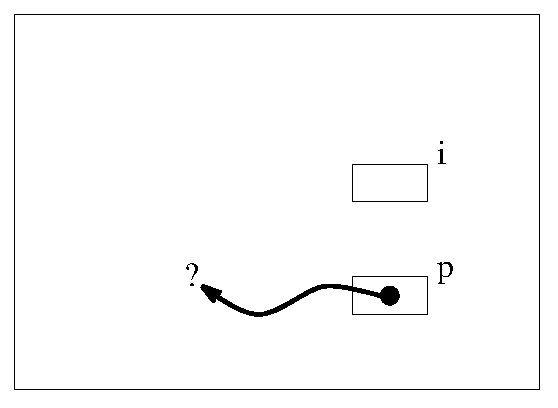
\includegraphics{../Figs/point8_1.eps}
}
\end{figure}
\end{center}
\vspace{-1in}
\section*{Assigment}
\begin{verbatim}
p = NULL;
\end{verbatim}
\begin{center}
\begin{figure}[h]
\centerline{
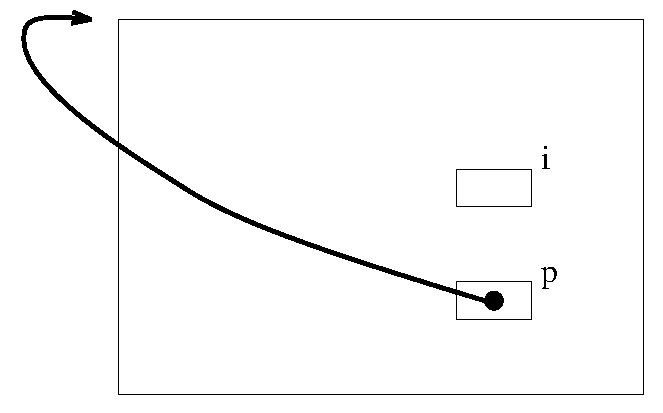
\includegraphics{../Figs/point8_2.eps}
}
\end{figure}
\end{center}
}
\newpage
{\samepage
\begin{verbatim}
p = &i;
\end{verbatim}
\begin{center}
\begin{figure}[h]
\centerline{
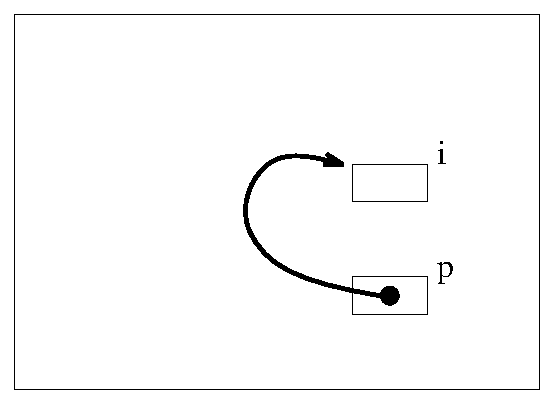
\includegraphics{../Figs/point8_3.eps}
}
\end{figure}
\end{center}
\begin{verbatim}
i = 5;
\end{verbatim}
\begin{center}
\begin{figure}[h]
\centerline{
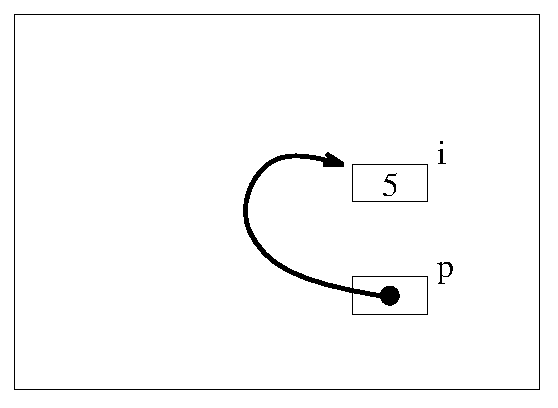
\includegraphics{../Figs/point8_4.eps}
}
\end{figure}
\end{center}
}

\newpage
\section*{Dereferencing Pointers}
\begin{verbatim}
printf("%d\n", *p);/* Dereference p */
\end{verbatim}
This prints \verb^5^.
\begin{verbatim}
i = 17;
printf("%d\n", *p);
\end{verbatim}
This prints \verb^17^.

\newpage
\begin{verbatim}
*p = 10;
\end{verbatim}
\begin{center}
\begin{figure}[h]
\centerline{
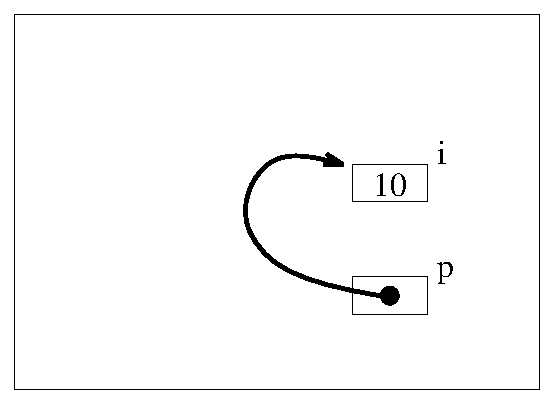
\includegraphics{../Figs/point8_5.eps}
}
\end{figure}
\end{center}
\begin{verbatim}
printf("%d\n", i);
\end{verbatim}
This prints \verb^10^.

\newpage
\section*{Back to {\tt scanf()}}
Using:
\begin{verbatim}
scanf("%d", &i);
\end{verbatim}
is now the same as:
\begin{verbatim}
scanf("%d", p);
\end{verbatim}
provided that \verb^p = &i^.

In many ways the dereference operator \verb^*^ is
the inverse of the address operator \verb^&^.

\newpage
\section*{Equivalence}
\begin{verbatim}
float x, y, *p;

p = &x;
y = *p;
\end{verbatim}
\begin{center}
\begin{figure}[h]
\centerline{
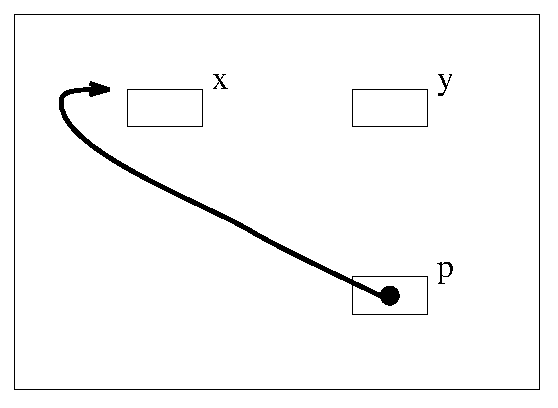
\includegraphics{../Figs/point8_6.eps}
}
\end{figure}
\end{center}
What is this equivalent to ?
\newpage
Pointers may be assigned when both sides have the same type:
\begin{verbatim}
int *p;
p = 10;           /* Illegal */
p = (int *) 10;   /*  Legal  */
\end{verbatim}


\newpage
\section*{The Swap Function}
{\small
\begin{verbatim}
#include <stdio.h>

void swap(int *p, int *q);

int main(void)
{
   int   a = 3, b = 7;

   /* 3 7 printed */
   printf("%d %d\n", a, b);
   swap(&a, &b);
   /* 7 3 printed */
   printf("%d %d\n", a, b);
   return 0;
}

void swap(int *p, int *q)
{
   int   tmp;

   tmp = *p;
   *p = *q;
   *q = tmp;
}
\end{verbatim}
}

\newpage
\section*{Dissecting {\tt swap()}}
When the function is called:
\begin{center}
\begin{figure}[h]
\centerline{
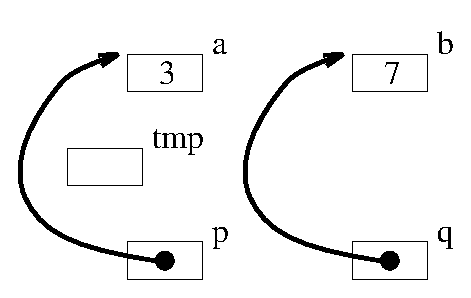
\includegraphics{../Figs/point8_7.eps}
}
\end{figure}
\end{center}
\begin{verbatim}
tmp = *p;
*p = *q;
*q = tmp;
\end{verbatim}
\begin{center}
\begin{figure}[h]
\centerline{
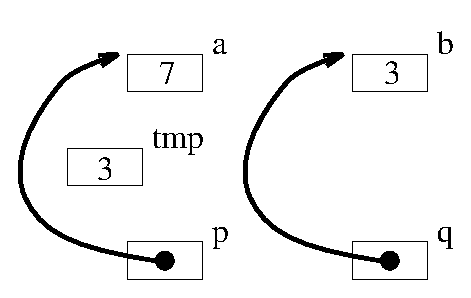
\includegraphics{../Figs/point8_8.eps}
}
\end{figure}
\end{center}

\newpage
\section*{Storage Classes}
\begin{itemize}
\item {\bf auto}
\begin{verbatim}
auto int a, b, c;
auto float f;
\end{verbatim}
Because this is the default, it is seldom used.

\item {\bf extern}

Tells the compiler to look for the variable elsewhere,
possibly another file.

\item {\bf register}

Informs the compiler to place the variable in a high-speed
memory register if possible,\\ i.e.\ if there are enough such
registers available \& the hardware supports this.

\item {\bf static}

Allows local variables to maintain their values :
\begin{verbatim}
void f(void)
{

   static int cnt = 0;

   cnt++;
}
\end{verbatim}
\end{itemize}

\newpage
\section*{Type Qualifiers}

\begin{itemize}
\item {\bf const}
\begin{verbatim}
const int k = 3;
\end{verbatim}
Once \verb^k^ is initialised, it cannot be changed in any way.

\item {\bf volatile}
{\small
\begin{verbatim}
extern const volatile int real_time_clock;
\end{verbatim}
}
Very rarely used, this variable may be changed by the {\it hardware}
in some unspecified way.
\end{itemize}

\newpage
{\samepage
\begin{center}
{\Large Chapter Nine \\ Arrays \& Pointers}
\end{center}

\newpage
\section*{One-Dimensional Arrays}
\begin{verbatim}
#include <stdio.h>

#define   N   5

int main(void)
{
   /* allocate space a[0]...a[4] */
   int   a[N];
   int   i, sum = 0;

   /* fill array */
   for (i = 0; i < N; ++i)
      a[i] = 7 + i * i;
   /* print array */
   for (i = 0; i < N; ++i)
      printf("a[%d] = %d", i, a[i]);
   /* sum elements */
   for (i = 0; i < N; ++i)
      sum += a[i];
   /* print sum */
   printf("\nsum = %d\n", sum);
   return 0;
}
\end{verbatim}
}
\newpage
\begin{itemize}
\item One-Dimensional arrays are declared by a type
followed by an identifier with a bracketed constant expression:
\vspace{-1em}
\begin{verbatim}
float x[10];
int k[ARRAY_SIZE];
\end{verbatim}
\vspace{-1em}
The following, however, is not valid:
\vspace{-1em}
\begin{verbatim}
float y[i*2];
\end{verbatim}
\vspace{-1em}
\item Arrays are stored in contiguous memory, e.g.:
\vspace{-1em}
\begin{verbatim}
int a[5];
\end{verbatim}
\vspace{-1em}
\begin{center}
\begin{figure}[h]
\centerline{
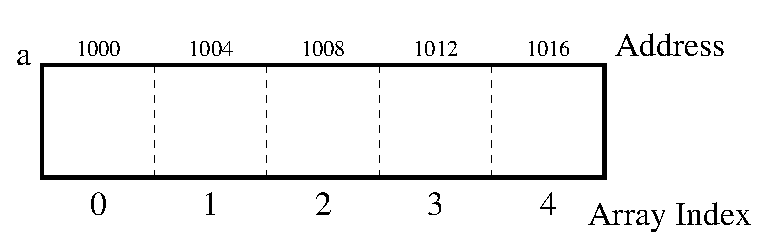
\includegraphics{../Figs/array9_1.eps}
}
\end{figure}
\end{center}
\item Arrays are indexed {\bf 0} to {\bf n-1}.
\end{itemize}
\newpage
\section{Initialisation}
By default, arrays are uninitialised.
When they are declared, they may be assigned a value:
{\small
\begin{verbatim}
float x[7] = {-1.1,0.2,2.0,4.4,6.5,0.0,7.7};
\end{verbatim}
}
or,
{\small
\begin{verbatim}
float x[7] = {-1.1, 0.2};
\end{verbatim}
}
the elements 2 ... 6 are set to zero.

Also:
{\small
\begin{verbatim}
int a[] = {3, 8, 9, 1};
\end{verbatim}
}
is valid, the compiler assumes the array size to be \verb^4^.


\newpage
\section*{Using Arrays}
\begin{itemize}
\item Accessing an array out of bounds will not be identified by
the compiler. It may cause an error at run-time.
One frequent result is that an entirely unrelated variable
is altered.
\item \verb^a[5] = a[4] + 1;^
\item \verb^k[9]++;^
\item \verb^n[12+i] = 0;^
\end{itemize}

\newpage
{\samepage
\begin{verbatim}
/* Count lowercase letters */
#include <stdio.h>
#include <ctype.h>

int main(void)
{
   int   c, i, letter[26];

   /*  zero   */
   for (i = 0; i < 26; ++i)
      letter[i] = 0;
   /*  count  */
   while ((c = getchar())!=EOF)
      if (islower(c))
         ++letter[c - 'a'];
   /* results */
   for (i = 0; i < 26; ++i) {
      if (i % 5 == 0)
         printf("\n");
      printf("%c:%4d  ", 'a' + i,
              letter[i]);
   }
   printf("\n\n");
   return 0;
}
\end{verbatim}
}
\newpage
The results of running the code on
the handout of lectures 1 to 7:
\begin{verbatim}
a: 840  b: 212  c: 436  d: 409  e:1449
f: 313  g: 173  h: 392  i:1112  j:   9
k:  34  l: 470  m: 373  n: 952  o: 666
p: 285  q:  21  r: 743  s: 696  t:1196
u: 398  v: 157  w:  97  x:  56  y: 148
z:  43
\end{verbatim}
\newpage
{\samepage
\section*{Arrays are Pointers ?}
\vspace{-1em}
An array name by itself is simply an address.
For instance:
\begin{verbatim}
int a[5];
int *p;
\end{verbatim}
declares an array of \verb^5^ elements, and
\verb^a^ is the address of the start of the
array.
Assigning:
\vspace{-1em}
\begin{verbatim}
p = a;
\end{verbatim}
\vspace{-1em}
is completely valid and
the same as:
\vspace{-1em}
\begin{verbatim}
p = &a[0];
\end{verbatim}

\begin{center}
\begin{figure}[ht]
\centerline{
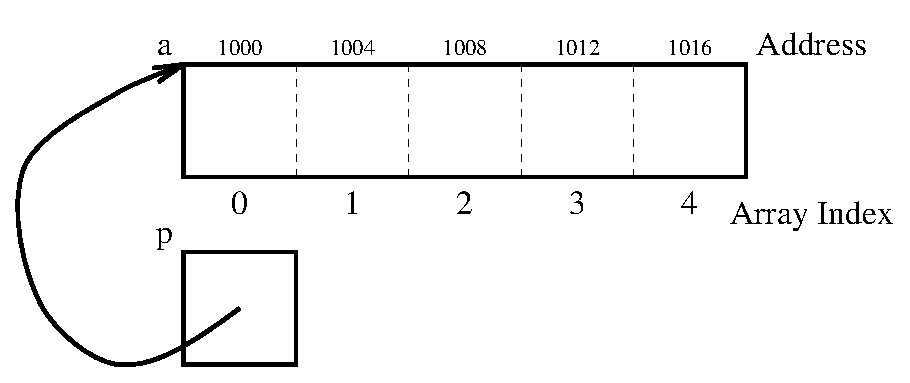
\includegraphics{../Figs/array9_2.eps}
}
\end{figure}
\end{center}
}
\newpage
{\samepage
To assign \verb^p^ to point to the next element,
we could use
\begin{verbatim}
p = a + 1;
\end{verbatim}
or
\begin{verbatim}
p = &a[1];
\end{verbatim}
\begin{itemize}
\item Notice that \verb^p = a + 1^ advances
the pointer {\bf 4} bytes and not 1 byte.
This is because an integer is 4 bytes long and
\verb^p^ is a pointer to an int.
\item we can use the pointer \verb^p^ is exactly
the same way as normal, i.e.:
\begin{verbatim}
*p = 5;
\end{verbatim}
\end{itemize}
}

\newpage
\section*{Summing an Array - 1}
\begin{verbatim}
#include <stdio.h>

int main(void)
{

   int a[] = {10, 12, 6, 7, 2};
   int i;
   int sum = 0;

   for(i=0; i<5; i++){
      sum += a[i];
   }
   printf("%d\n", sum);

   return 0;

}
\end{verbatim}

\newpage
\section*{Summing an Array - 2}
\begin{verbatim}
#include <stdio.h>

int main(void)
{

   int a[] = {10, 12, 6, 7, 2};
   int i;
   int sum = 0;

   for(i=0; i<5; i++){
      sum += *(a + i);
   }
   printf("%d\n", sum);

   return 0;

}
\end{verbatim}

\newpage
\section*{Summing an Array - 3}
\begin{verbatim}
#include <stdio.h>

int main(void)
{

   int a[] = {10, 12, 6, 7, 2};
   int i;
   int sum = 0;
   int *p;

   p = a;
   for(i=0; i<5; i++){
      sum += *p;
      p++;
   }
   printf("%d\n", sum);

   return 0;

}
\end{verbatim}
\newpage
\section*{Passing Arrays to Functions}
When an array is passed to a function, what
is actually passed is a pointer to the base address,
not a copy of the array itself.
\begin{verbatim}
#include <stdio.h>

void zero_array(int b[], int s);
void zero_array2(int *b, int s);

int main(void)
{

   int a[5]; /* Uninitialised */

   zero_array(a, 5);
   return 0;

}
\end{verbatim}
\newpage
\begin{verbatim}
void zero_array(int b[], int s)
{

   int i;
   for(i=0; i<s; i++)
      b[i] = 0;
}

void zero_array2(int *b, int s)
{

   int i;
   for(i=0; i<s; i++)
      *b++ = 0;
}
\end{verbatim}
To initialise the middle three elements we could have called:
\begin{verbatim}
zero_array(&a[1], 3);
\end{verbatim}

\newpage
\section*{The Bubblesort}
\begin{verbatim}
#include <stdio.h>

void bubble_sort(int b[], int s);

int main(void)
{

   int i;
   int a[] = {3, 4, 1, 2, 9, 0};

   bubble_sort(a, 6);

   for(i=0; i<6; i++){
      printf("%d ", a[i]);
   }
   printf("\n");

   return 0;

}
\end{verbatim}
\newpage
\begin{verbatim}
void bubble_sort(int b[], int s)
{

   int i, tmp;
   int changes;

   do{
      changes = 0;
      for(i=0; i<s-1; i++)
         if(b[i] > b[i+1]){
            tmp = b[i];
            b[i] = b[i+1];
            b[i+1] = tmp;
            changes++;
         }
   }while(changes);
}
\end{verbatim}
\newpage

During each pass, the array contains:
\begin{verbatim}
3 1 2 4 0 9
1 2 3 0 4 9
1 2 0 3 4 9
1 0 2 3 4 9
0 1 2 3 4 9
0 1 2 3 4 9
\end{verbatim}

\newpage
\section*{Two-Dimensional Arrays}
A 2D array is declared as follows:
\begin{verbatim}
#define ROWS 3
#define COLS 5
int a[ROWS][COLS];
\end{verbatim}
\begin{center}
\begin{tabular}{|l|l|l|l|l|l|} \hline
    &   col 1   & col 2 & col 3 & col 4 & col 5 \\ \hline
row 1   & a[0][0]   & a[0][1]   & a[0][2]   & a[0][3]   & a[0][4] \\
row 2   & a[1][0]   & a[1][1]   & a[1][2]   & a[1][3]   & a[1][4] \\
row 3   & a[2][0]   & a[2][1]   & a[2][2]   & a[2][3]   & a[2][4] \\ \hline
\end{tabular}
\end{center}
 2D array initialisation :
\begin{verbatim}
int a[2][3] = {1, 2, 3, 4, 5, 6};
int a[2][3] = {{1, 2, 3}, {4, 5, 6}};
int a[ ][3] = {{1, 2, 3}, {4, 5, 6}};
\end{verbatim}

\newpage
Although \verb^a^ is stored in a contiguous block of memory,
we may think of it as a 2D rectangle of data.
\begin{center}
\begin{figure}[h]
\centerline{
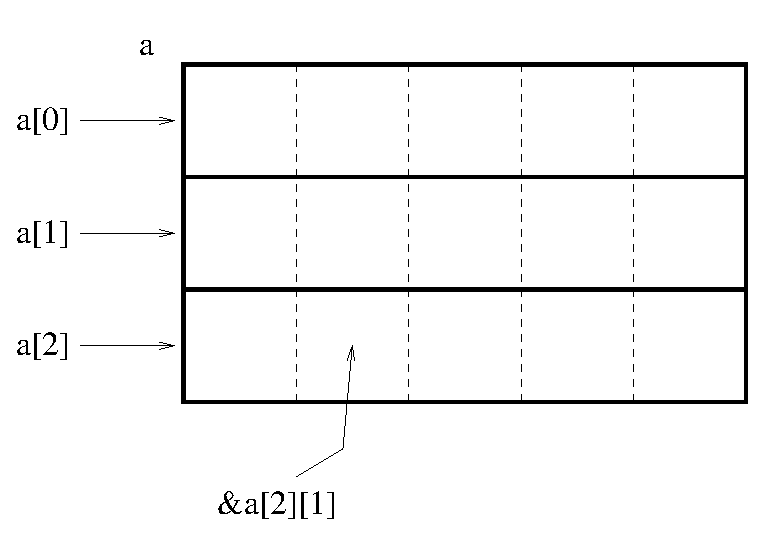
\includegraphics{../Figs/array9_3.eps}
}
\end{figure}
\end{center}
\verb^a[i][j]^ is equivalent to:\\
\verb^*(a[i] + j)^\\
\verb^(*(a + i))[j]^\\
\verb^*((*(a + i)) + j)^\\
\verb^*(&a[0][0] + 5*i + j)^


\newpage
\begin{verbatim}
#include <stdio.h>

/* number of rows */
#define   M   3
/* number of columns */
#define   N   4

int main(void)
{
   int   a[M][N], i, j, sum = 0;

   putchar('\n');
   /* fill array */
   for (i = 0; i < M; ++i)
      for (j = 0; j < N; ++j)
         a[i][j] = i + j;
   /* array values */
   for (i = 0; i < M; ++i){
      for (j = 0; j < N; ++j)
         printf("a[%d][%d] = %d ",
                 i, j, a[i][j]);
      printf("\n");
   }
   /* sum the array */
   for (i = 0; i < M; ++i)
      for (j = 0; j < N; ++j)
         sum += a[i][j];
   printf("\nsum = %d\n\n", sum);
   return 0;
}
\end{verbatim}

\newpage
\section*{Dynamic Memory}
In some cases the size of an array may not be known.
The size may be decided by the user, or by a computation.
There are two functions which provide the ability to
dynamically allocate memory:
\begin{verbatim}
void *calloc(num_els, el_size);
void *malloc(num_bytes);
\end{verbatim}
Both functions return pointers.
\verb^calloc()^ initialises its memory to
zero, whereas \verb^malloc()^ does not.
If \verb^NULL^ is returned, then the allocation
has failed.

The file \verb^stdlib.h^ contains definitions and prototypes
required to use the functions.

The function:\\
\verb^void free(void *ptr);^\\
frees the memory once it is no longer required.

\newpage
\begin{verbatim}
/* To allocate 256 bytes of memory */
#include <stdio.h>
#include <stdlib.h>

int main(void)
{

   int *p;

   p = (int *)malloc( 256 );

   if(p == NULL){
      printf("Allocation Failed...\n");
      exit(EXIT_FAILURE);
   }

   return(0);

}
\end{verbatim}


\newpage
\begin{center}
{\Large Chapter Ten \\ Strings \& Pointers}
\end{center}
\vspace{-0.5in}
\section*{Strings}
\begin{itemize}
\item Strings are 1D arrays of characters.
\item Any character in a string may be accessed as an array
element, or by dereferencing a pointer.
\item The important difference between strings and ordinary arrays
is the {\bf end-of-string sentinel} \verb^'\0'^ or null character.
\end{itemize}

\newpage
\begin{itemize}
\item The string "abc" has a {\it length} of 3, but its {\it size} is 4.
\item Note \verb^'a'^ and \verb^"a"^ are different. The first is a
character constant, the second is a string with 2 elements
\verb^'a'^ and \verb^'\0'^.
\end{itemize}

\newpage
\section*{Initialising Strings}
\begin{itemize}
\item \begin{verbatim}
char w[250];
w[0] = 'a';
w[1] = 'b';
w[2] = 'c';
w[3] = '\0';
\end{verbatim}
\item \begin{verbatim}
scanf("%s", w);
\end{verbatim}
Removes leading spaces, reads a string (terminated by a
space or \verb^EOF^). Adds a null character to the end
of the string.
\item \begin{verbatim}
char w[250] = {'a', 'b', 'c', '\0'};
\end{verbatim}
\end{itemize}

\newpage
{\samepage
\begin{itemize}
\item \begin{verbatim}
char w[250] = "abc";
\end{verbatim}
\item \begin{verbatim}
char *w = "abc";
\end{verbatim}
\end{itemize}
\begin{verbatim}

#include <stdio.h>
#include <ctype.h>

int main(void)
{
   char w1[100] = "test";
   char *w2 = "test";

   printf("%s -> ", w1);
   w1[0] = toupper(w1[0]);
   printf("%s\n", w1);

   printf("%s -> ", w2);
   /* Seg Faults */
   w2[0] = toupper(w2[0]);
   printf("%s\n", w2);

   return 0;
}
\end{verbatim}
}

\newpage
{\samepage
\section*{Repeated Characters}
{\small
\begin{verbatim}
#include <stdio.h>
#include <ctype.h>

int main(void)
{

   char s[100] =
      "The Quick Brown Fox Leaps " \
      "Over the Lazy Dog";
   short used[26] = {0};
   char c;
   int i = 0;

   while(s[i]){
      c = tolower(s[i]);
      if(islower(c)){
         used[c - 'a'] = 1;
      }
      i++;
   }

   for(i=0; i<26; i++)
      if(!used[i])
         printf("%c has not been used.\n",
                i+'a');

   return 0;

}
\end{verbatim}

Output:
\begin{verbatim}
j has not been used.
m has not been used
\end{verbatim}
}
}
\newpage
{\samepage
\section*{Pointers \& String Processing}
\begin{verbatim}
/* Character processing:
   change a line.        */

#include <stdio.h>

#define   MAXLINE   100

char   *change(char *s);
void   read_in(char s[]);

int main(void)
{
   char   line[MAXLINE];

   printf("\nWhat is your " \
          "favourite line? ");
   read_in(line);
   printf("\n%s\n\n%s\n\n",
    "Here it is after being changed:",
    change(line));
   return 0;
}
\end{verbatim}
}
\newpage
{\samepage
\begin{verbatim}
void read_in(char s[])
{
   int    c, i = 0;

   while ((c = getchar()) != EOF &&
           c != '\n')
      s[i++] = c;
   s[i] = '\0';
}

char *change(char *s)
{
   static char   new_string[MAXLINE];
   char          *p = new_string;

   *p++ = '\t';
   for ( ; *s != '\0'; ++s)
      if (*s == 'e')
       *p++ = 'E';
      else if (*s == ' ') {
       *p++ = '\n';
       *p++ = '\t';
      }
      else
       *p++ = *s;
   *p = '\0';
   return new_string;
}
\end{verbatim}
}
\newpage
{\samepage
\section*{Dissection}
\begin{verbatim}
What is your favourite line?
she sells sea shells

Here it is after being changed:

        shE
        sElls
        sEa
        shElls
\end{verbatim}
\begin{itemize}
\item Every \verb^e^ changes to \verb^E^, every space swapped
with a newline and tab.
\item In \verb^read_in()^ we assume less than \verb^MAXLINE^ characters
are entered. We could use an\\ \verb^assert()^ here.
\item Note the use of \verb^static^ in \verb^change()^.
\item \verb^*p++^ is equivalent to \verb^*(p++)^ and {\bf not}
\verb^(*p)++^.
\end{itemize}
}
\newpage
\section*{String Handling Functions}
In \verb^#include <string.h>^ :
{\small
\begin{verbatim}
char *strcat(char *dst, const char *src);
int strcmp(const char *s1, const char *s2);
char *strcpy(char *dst, const char *src);
unsigned strlen(const char *s);
\end{verbatim}
}
\begin{itemize}
\item \verb^strcat()^ appends a copy of string \verb^src^,
including  the  terminating null character,
to  the  end  of  string  \verb^dst^.
\item \verb^strcmp()^ compares two strings byte-by-byte, according to the
     ordering  of  your  machine's  character  set.  The function
     returns an integer greater than, equal to, or less  than  0,
     if the string pointed to by \verb^s1^ is greater than, equal to, or
     less than the string pointed to by \verb^s2^ respectively.
\item \verb^strcpy()^ copies string \verb^src^ to \verb^dst^
including the  terminating null  character,
stopping after the null character has been copied.
\item \verb^strlen()^ returns the number of bytes in \verb^s^,
not including the terminating null character.
\end{itemize}

\newpage
\section*{The Function {\tt strlen()}}
One way to write the function \verb^strlen()^
\begin{verbatim}
unsigned strlen(const char *s)
{

   register int n = 0;

   for(; *s != '\0'; ++s)
      ++n;
   return n;
}
\end{verbatim}

\newpage
\begin{center}
{\Large Chapter Twelve\\ Structures}
\end{center}
\vspace{-1.0in}
\section*{Declaring Structures}
\begin{itemize}
\item A structure type allows the programmer to aggregate components
into a single, named variable.
\item Each component has individually named members.
\item \begin{verbatim}
struct card {
   int pips;
   char suit;
};
\end{verbatim}
\item \verb^struct^ is a keyword, \verb^card^ is the structure
tag name, and \verb^pips^ and \verb^suit^ are members of the structure.
\end{itemize}

\newpage
\begin{itemize}
\item A statement of the form :\\
\verb^struct card c1, c2;^\\
actually creates storage for identifiers
\item A member is accessed using the member operator ``.''
\item
\begin{verbatim}
c1.pips = 5;
c1.suit = 'd';
c2.pips = 12;
c2.suit = 's';
\end{verbatim}
\item The member name must be unique within the same structure.
\end{itemize}
\newpage
\begin{itemize}
\item We can declare the structure and variables in one statement:
\begin{verbatim}
struct card {
   int pips;
   char suit;
} c1, c2;
\end{verbatim}
\item In the above, \verb^card^ is optional.
\item Arrays of structures are possible, i.e.:
\begin{verbatim}
struct card pack[52];
\end{verbatim}
\end{itemize}

\newpage
{\samepage
{\small
\begin{verbatim}
#include <stdio.h>
#include <ctype.h>

struct student {
   char *surname;
   int id;
   char grade;
};

int failures(struct student j[], int n);

int main(void)
{
   struct student class[] = {
      {"Bloggs",    95112174, 'c'},
      {"Doobeedoo", 96162578, 'b'},
      {"Campbell",  96112103, 'f'},
      {"Johnson",   96185617, 'a'}
   };
   printf("Number of fails : %d\n",
          failures(class, 4));
   return 0;
}

int failures(struct student j[], int n)
{

   int i, cnt = 0;

   for(i=0; i<n; i++)
      cnt += (tolower(j[i].grade) == 'f');
   return cnt;
}
\end{verbatim}
}}
\newpage
\section*{Structures \& Pointers}
\begin{itemize}
\item \verb^struct student *p;^\\
declares a pointer to a structure.
\item Point it at something sensible:\\
\verb^p = &c1;^
\item Now we access its members using the ``\verb^->^''
operator.
\item \verb^p->id = 96123040;^
\item The deference, followed by the member access, could also be written as: \verb^(*p).id = 96123949;^
\end{itemize}

\newpage
{\samepage
{\small
\begin{verbatim}
#include <stdio.h>
#include <ctype.h>

struct student {
   char *surname;
   int id;
   char grade;
};

int failures(struct student *j, int n);

int main(void)
{
   struct student class[] = {
      {"Bloggs",    95112174, 'c'},
      {"Doobeedoo", 96162578, 'b'},
      {"Campbell",  96112103, 'f'},
      {"Johnson",   96185617, 'a'}
   };

   printf("Number of fails : %d\n",
          failures(class, 4));
   return 0;
}

int failures(struct student *j, int n)
{
   int i, cnt = 0;
   for(i=0; i<n; i++){
      cnt += (tolower(j->grade) == 'f');
      j++;
   }
   return cnt;
}
\end{verbatim}
}}
\newpage
{\samepage
{\small
\begin{verbatim}
/* Nested Structures */
#include <stdio.h>

struct date {
   short day;
   short month;
   short year;
};

struct person {
   char name[25];
   struct date date;
};

void print_person_copy(struct person p);
void print_person_point(struct person *p);

int main(void)
{

   struct person k;

   printf("Enter your surname : ");
   scanf("%s", k.name);
   printf("Enter your Birthday: ");
   scanf("%hd/%hd/%hd", &k.date.day,
         &k.date.month, &k.date.year);

   print_person_copy(k);
   print_person_point(&k);

   return 0;
}
\end{verbatim}
}}
\newpage
{\small
\begin{verbatim}

void print_person_copy(struct person p)
{

   printf("Name \"%s\", Born " \
          "%02d/%02d/%d\n",
      p.name, p.date.day,
      p.date.month, p.date.year);

}

void print_person_point(struct person *p)
{

   printf("Name \"%s\", Born " \
          "%02hd/%02hd/%hd\n",
      p->name, p->date.day,
      p->date.month, p->date.year);

}
\end{verbatim}
}
\begin{verbatim}
Enter your surname : Campbell
Enter your Birthday: 8/12/68
Name "Campbell", Born 08/12/68
Name "Campbell", Born 08/12/68
\end{verbatim}

\newpage
\section*{Self-Referential Structures}
\begin{verbatim}
struct list {
   int data;
   struct list *next;
};
\end{verbatim}
\begin{itemize}
\item The pointer variable \verb^next^ is called a {\bf link}.
\item \begin{verbatim}
struct list a, b, c;
a.data = 1;
b.data = 2;
c.data = 3;
a.next = b.next = c.next = NULL;
\end{verbatim}
\begin{center}
\begin{figure}[h]
\centerline{
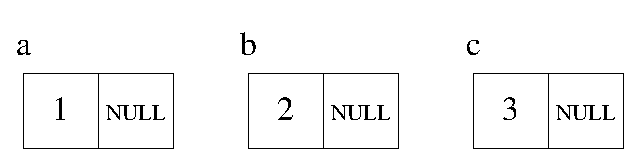
\includegraphics{../Figs/link1.eps}
}
\end{figure}
\end{center}
\end{itemize}
\newpage
\begin{itemize}
\item \begin{verbatim}
a.next = &b;
b.next = &c;
\end{verbatim}
\begin{center}
\begin{figure}[h]
\centerline{
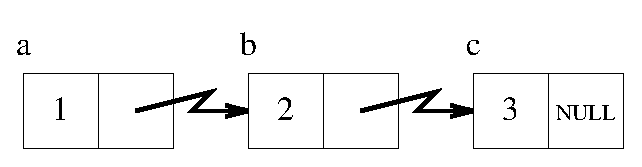
\includegraphics{../Figs/link2.eps}
}
\end{figure}
\end{center}
\item \begin{verbatim}
/* has value 2 */
a.next -> data;
/* has value 3 */
b.next -> data;
/* has value 3 */
a.next -> next -> data;
\end{verbatim}
\end{itemize}

\newpage
\section*{Dynamic List Creation}
\begin{itemize}
\item We may need to dynamically create objects in a linked
list, using \verb^malloc()^.
\item \verb^malloc(sizeof(list));^ returns a pointer
to a new, free block of memory.
\item Need to be able to Add/Delete/Count/Insert elements.
\end{itemize}

\newpage
{\samepage
{\small
\begin{verbatim}
#include <stdio.h>
#include <stdlib.h>
#include <string.h>

#define BIGGESTNAME 50

struct llist {
   char word[BIGGESTNAME];
   struct llist *next;
};

int main(void)
{
   struct llist *head, *cp;

   printf("Enter a list of words.\n");
   cp = head = calloc(1, sizeof(struct llist));
   while(scanf("%s", cp->word)==1){
      cp->next = calloc(1, sizeof(struct llist));
      cp = cp->next;
   }

   cp = head;
   printf("The words were :\n");
   while(cp->next != NULL){
      printf("%s\n", cp->word);
      cp = cp->next;
   };
   return 0;
}
\end{verbatim}
}}

\newpage
\begin{center}
{\Large Chapter Thirteen\\ File Handling}
\end{center}
\section*{File Properties}
Files have many important properties:
\begin{itemize}
\item They have a name.
\item Until a file is opened nothing can be done with it.
\item After use a file must be closed.
\item Files may be read, written or appended.
\item Conceptually a file may be thought of as a stream of characters.
\end{itemize}

\newpage
\section*{Accessing Files}
\vspace{-0.75em}
\begin{verbatim}
#include <stdio.h>

int main(void)
{

   int sum = 0, val;
   FILE *ifp, *ofp;

   /* Read a File */
   ifp = fopen("my_file", "r");
   /* Write to a File */
   ofp = fopen("outfile", "w");

     .
     .
     .

   fclose(ifp);
   fclose(ofp);
}
\end{verbatim}
\vspace{-0.75em}
\newpage
\section*{Opening Files}
\vspace{-0.75em}
{\small
\begin{verbatim}
FILE *fopen(char *filename, char *modes);
\end{verbatim}
}
\vspace{-0.75em}
The mode for file opening is a {\it string}, and can
take the following options:
\begin{center}
\begin{tabular}{|l|l|}\hline
``r''  & open text file for reading \\ \hline
``w''  & open text file for writing \\ \hline
``a''  & open text file for appending\\ \hline
``rb'' & open binary file for reading \\ \hline
``wb''  & open binary file for writing\\ \hline
``ab''  & open binary file for appending\\ \hline
\end{tabular}
\end{center}
If the file cannot be found, or if it is not readable,
then the function returns \verb^NULL^.
\vspace{-0.75em}
\begin{verbatim}
fp = fopen("filedoof", "r");
if(fp == NULL){
   exit(EXIT_FAILURE);
}
\end{verbatim}

\newpage
\section*{Getting \& Putting Characters}
The functions \verb^fgetc()^ and \verb^fputc()^ are
similar to \verb^getchar()^ and \verb^putchar()^, but
additionally take a file pointer as an argument.
\vspace{-0.75em}
\begin{verbatim}
int fgetc(FILE *stream);
int fputc(int c, FILE *stream);
\end{verbatim}

\newpage
{\samepage
\vspace*{-1in}
\begin{small}
\begin{verbatim}
/* Number the lines of a file */
#include <stdio.h>

int main(void)
{

   FILE *fp;
   char fname[128];
   char str[500];
   int i, c, line;

   printf("What file would you like to see ? ");
   scanf("%s", fname);
   if((fp = fopen(fname, "r")) == NULL){
      printf("Cannot open file\n");
      exit(EXIT_FAILURE);
   }
   line = 1;
   do{
      i = 0;
      do{
         c = (str[i++] = fgetc(fp));
      }while(c != EOF && c != '\n');
      str[i] = '\0';
      if(c != EOF){
         printf("%5d %s", line, str);
         line++;
      }
   }while(c != EOF);
   fclose(fp);

   return 0;
}
\end{verbatim}
\end{small}
}

\newpage
{\samepage
\vspace*{-1in}
\begin{small}
\begin{verbatim}
/* Copying Files */
#include <stdio.h>
#include <stdlib.h>

#define MAXFILENAME 128

int main(void)
{

   FILE *ifp, *ofp;
   char inpname[MAXFILENAME];
   char oupname[MAXFILENAME];
   int i;

   printf("Enter two filenames : ");
   if(scanf("%s %s", inpname, oupname) != 2){
      printf("Failed to scan two filenames.");
      exit(EXIT_FAILURE);
   }
   ifp = fopen(inpname, "rb");
   ofp = fopen(oupname, "wb");
   if(ifp == NULL || ofp == NULL){
      printf("Failed to open two filenames.");
      exit(EXIT_FAILURE);
   }
   while((i = fgetc(ifp)) != EOF){
      fputc(i, ofp);
   };

   fclose(ifp);
   fclose(ofp);

   return 0;

}
\end{verbatim}
\end{small}
}
\newpage
\section*{Reading / Writing Data Blocks}
The functions \verb^fread()^ and \verb^fwrite()^ allow
blocks of information to be read and written using files.
\begin{small}
\begin{verbatim}
fread(void *ptr, size, num_items, stream);
fwrite(void *ptr, size, num_items, stream);
\end{verbatim}
\end{small}
\vspace{-0.25em}
They return an unsigned integer, the number of elements correctly
read or written.

\newpage
{\samepage
\vspace*{-1in}
\begin{small}
\begin{verbatim}
#include <stdio.h>
#include <stdlib.h>

struct examp {
   int h[100];
   double k;
   char c;
};
typedef struct examp examp;

int main(void)
{

   FILE *fp;
   examp e;
   printf("%d\n", sizeof(double));
   if((fp = fopen("doof", "rb")) == NULL){
      printf("Cannot read file\n");
      exit(EXIT_FAILURE);
   }
   /* Should check return from fread */
   fread(&e, sizeof(struct examp), 1, fp);
   printf("k = %f\n", e.k);
   fclose(fp);
    .
    .
    .
   if((fp = fopen("doof", "wb")) == NULL){
      printf("Cannot write file\n");
      exit(EXIT_FAILURE);
   }
   /* Should check return from fwrite */
   fwrite(&e, sizeof(struct examp), 1, fp);
   fclose(fp);
   return 0;
}
\end{verbatim}
\end{small}
}
\newpage
\section*{Printing and Scanning Files}
The functions:
{\small
\begin{verbatim}
int fprintf(FILE *stream, format, other args);
int fscanf(FILE *stream, format, other args);
\end{verbatim}
}
act almost the same as their \verb^printf()^ and \verb^scanf()^
counterparts, except that input is from file rather than keyboard.

\newpage
\begin{small}
\begin{verbatim}
#include <stdio.h>
#include <stdlib.h>

int main(void)
{

   FILE *fp;

   if((fp = fopen("file.txt", "w")) == NULL){
      printf("Cannot open file\n");
      exit(EXIT_FAILURE);
   }
   fprintf(fp, "Hello World\n");
   fclose(fp);

   return 0;
}
\end{verbatim}
\end{small}
Creates a file called \verb^file.txt^ with the
string \verb^Hello World^ in it.

\newpage
\section*{Stdout and Stderr}
On Unix systems, there are three pre-defined streams,
\verb^stdin^, \verb^stdout^ and \verb^stderr^. Since
\verb^stdin^ is the standard input stream, \verb^scanf()^ is
simply as special case of \verb^fscanf()^.
\begin{verbatim}
scanf("%d", &i);
fscanf(stdin, "%d", &i);
\end{verbatim}
Likewise, \verb^printf()^ is a special case of \verb^fprintf()^:
\begin{verbatim}
printf("%s %d", "The number is", i);
fprintf(stdout, "%s %d",
        "The number is", i);
\end{verbatim}
For printing error messages use:
\begin{verbatim}
fprintf(stderr, "Cannot open file %s",
        fname);
exit(EXIT_FAILURE);
\end{verbatim}
Even if \verb^stdout^ is being re-directed to a file, this
message will appear on the screen.

\newpage
\section*{Advanced {\tt scanf()}}
It is possible to specify a {\it scan set} when using\\
\verb^scanf()^ to input a string. For instance:
\vspace{-0.75em}
\begin{verbatim}
scanf("%[abc]s", str);
\end{verbatim}
\vspace{-0.75em}
allows you to read in a string containing the characters
\verb^a^,
\verb^b^ or
\verb^c^.
The string is terminated by any other character, so:
\vspace{-0.75em}
\begin{verbatim}
Please type a string : abacus
I scanned : abac
\end{verbatim}
\vspace{-0.75em}
A circumflex is used to specify only characters {\it not} in
the scan set.
\vspace{-0.75em}
\begin{verbatim}
scanf("%[^k]s", str);
\end{verbatim}
\vspace{-0.75em}
leads to every possible character other than \verb^'k'^ being
used in the scan set.
\vspace{-0.75em}
\begin{verbatim}
Please type a string : I Am Crackers
I scanned : I Am Crac
\end{verbatim}
\vspace{-0.75em}
\newpage
\section*{The {\tt sprintf()} Function}
This is very similar to the function \verb^printf()^, except
that the output is stored in a string rather than written
to the output.
It is defined as:
\vspace{-0.75em}
{\small
\begin{verbatim}
int sprintf(string, control-arg, other args);
\end{verbatim}
}
\vspace{-0.75em}
For example:
\vspace{-0.75em}
\begin{verbatim}
   int i = 7;
   float f = 17.041;
   char str[100];
   sprintf(str, "%d %f", i, f);
   printf("%s\n", str);

Outputs : 7 17.041000
\end{verbatim}
\vspace{-0.75em}
This is useful if you need to create a string for passing
to another function for further processing.

\newpage
\section*{The {\tt sscanf()} Function}
This is similar to the \verb^scanf()^ function, except
that the input comes from a string rather than from the keyboard.
It is defined as:
\vspace{-0.75em}
{\small
\begin{verbatim}
int sscanf(char *s, char *format, other args);
\end{verbatim}
}
\vspace{-0.75em}
For example:
\vspace{-0.75em}
\begin{small}
\begin{verbatim}
#include <stdio.h>
#include <stdlib.h>

#define STRLN 100

int main(void)
{

   char str[STRLN];
   int i;
   fgets(str, STRLN, stdin);
   while(sscanf(str, "%d", &i) != 1){
      printf("Cannot scan string !\n");
      fgets(str, STRLN, stdin);
   }
   printf("The number was %d.", i);

   return 0;
}
\end{verbatim}
\vspace{-0.75em}
\end{small}

\newpage
{\samepage
\section*{IO Summary}
\vspace{-1.5em}
{\large \bf Keyboard\\}
\vspace{-1.75em}
\begin{verbatim}
scanf(), getchar()
\end{verbatim}
{\large \bf Screen\\}
\vspace{-1.5em}
\begin{verbatim}
printf(), putchar()
\end{verbatim}
{\large \bf Output to File\\}
\vspace{-1.5em}
\begin{verbatim}
fprintf(), fputc(), fwrite()
\end{verbatim}
{\large \bf Input from File\\}
\vspace{-1.5em}
\begin{verbatim}
fscanf(), fgetc(), fread()
\end{verbatim}
{\large \bf Output to String}
\vspace*{-1.5em}
\begin{verbatim}
sprintf()
\end{verbatim}
{\large \bf Input from String}
\vspace*{-1.5em}
\begin{verbatim}
sscanf()
\end{verbatim}
}



\newpage
\section*{Common Errors}
\begin{itemize}
\item \verb^fopen("myfile", 'r');^
\item \verb^double d; scanf("%f", &d);^
\item Not using \verb^fclose()^
\item Every time \verb^sscanf()^ is called, scanning begins
at the start of the string, unlike \verb^fscanf()^ where
a record is kept of how far through the file we are.
\end{itemize}

\end{document}
